%%%%%%%%%%%%%%%%%%%%%%%%%%%%%%%%%%%%%%%%%
% University/School Laboratory Report
% LaTeX Template
% Version 2.0 (4/12/12)
%
% This template has been downloaded from:
% http://www.latextemplates.com
%
% License:
% CC BY-NC-SA 3.0 (http://creativecommons.org/licenses/by-nc-sa/3.0/)
%
% Original header:
%
%
%%%%%%%%%%%%%%%%%%%%%%%%%%%%%%%%%%%%%%%%%

%----------------------------------------------------------------------------------------
%	DOCUMENT CONFIGURATIONS
%----------------------------------------------------------------------------------------

\documentclass{article}

\usepackage{graphicx} % Allows the inclusion of images

\title{Custom Neurons Interface\\Developper Documentation} % Title

\author{Jonny \textsc{Quarta}} % Author name

\date{\today} % Specify a date for the report

\begin{document}

\maketitle % Insert the title, author and date


\setlength\parindent{0pt} % Removes all indentation from paragraphs

\renewcommand{\labelenumi}{\alph{enumi}.} % Make numbering in the enumerate environment by letter rather than number (e.g. section 6)

\section{Introduction}
The NEST Simulator, which stands for Neural Simulation Tool, has been created with the purpose of enabling complex simulations of point-like neurons. There's a wide range of possible models, from the simple integrate and fire model, to the more complex Hodgkin-Huxley one.\\
These neurons can be connected throught weighted connexions and their activity recorded using virtual tools (multimeter, spike detector, etc...).\\

In the NEST code, every model extends from a parent class, implementing only basic functions, such as collecting the incoming spikes. The real model is written in the child classes, so that, using polymorphism, adding new neurons is accomplished relatively easily.\\
However, each time one wants to add a new neuron, he has to write it in C++ (a difficult language) and recompile the whole project. This makes the tool not so flexible and slows down developpement time.\\
That's why the need for a plugin system has arised. This new feature should enable to easily write neurons, create .so files (shared libraries) and just put them in a special directory, which the NEST will automatically recognize and allow the code inside to be executed. In addition, since C++ is a difficult language, models should be written in a more scientific language such as Python.\\ \\
The purpose of this Bachelor Project is the creation of a plugin system having these features. This is accomplished using a relatively new technology, Cython. This special tool enables one to write Python code and compile it into C++.\\
During the next sections, first the NEST structure will be presented, then a global description of the NEST-.so file interface will be depicted. After that, more details are given, beginning with the NEST C++ side, followed by the CyNEST (the Cython) side. The next step will be a very little description of a tool used in order to compile the custom python neuron, \emph{cmpneuron}. Finally, performances and improvements are analyzed.

\section{NEST Structure}
The aim of this section is to enable the reader understanding the global NEST structure, which is essential in order to grasp the details of the new interface, presented in the next sections.\\
Basically NEST is composed of three major parts:
\begin{itemize}
\item The simulation kernel : this is the core of the system, enabling, among others, simulations, events scheduling, communication of neurons and activity recording. The C++ models are also situated in this part.
\item SLI Interface : NEST is a high configurable simulator, therefore a powerfull language has been created in order to configure simulation properties, set experiment parameters, create neurons and connexions between them, ect... SLI is loosely based on PostScript, using a stack to put, manipulate and retrieve objects.
\item CyNEST Interface : NEST can be used from a Python terminal, configuring it by calling very high functions, which will in turn call corresponding SLI commands. This interface can be accessed by just typing \emph{import cynest} in a Python terminal.
\end{itemize}
For more information, see the original documentation\\ (http://www.nest-initiative.org/index.php/Software:About\_NEST).

\section{Global Interface Structure}
This section deals with the global structure of the new interface between NEST and custom neurons. 

\begin{figure}[h]
\begin{center}
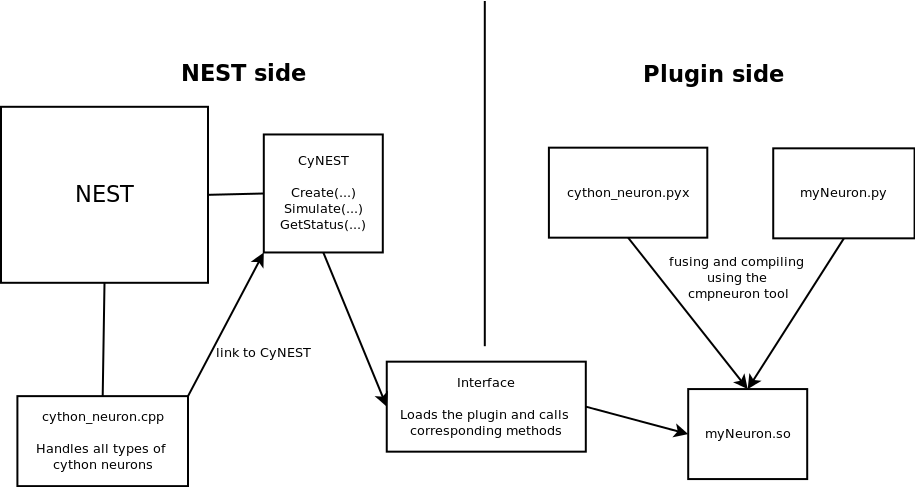
\includegraphics[width=0.92\textwidth]{Ressources/Interface_Structure}
\caption{Interface Structure}
\end{center}
\end{figure}

Figure 1 shows that structure as a diagram. One can see that there's a direct link between cython\_neuron.cpp and CyNEST (normally the two parts cannot directly communicate, but a link is necessary, that's why it has been added). The interface is placed between CyNEST and the plugin. \\
Let's admit that during a simulation, the update method of a neuron is called (a very likely situation!) and that this neuron is a custom one. The information flow is the following: NEST calls the update method of cython\_neuron.cpp, which through the direct link calls the CyNEST update function. This one uses the interface to call the previously loaded neuron update method inside that plugin file. We can actually say the CyNEST update method is somehow already a part of the interface.\\
During the next sections, the most important regions of the diagram will be covered in much greater detail, so that the reader can have insight into the subtle details and concepts that populate this innovative feature of NEST.

\section{C++ Side}
The fourth section of this document will describe in greater detail the implementation of the general cython neuron handler class, which is responsible for creating new neurons of a certain custom type, handling general events and calling the corresponding plugin functions (calibrate, update, ect...).

\subsection{Neuron Registration}
When creating a new neuron object in the Python terminal by typing\\ \emph{cynest.Create("myneuron")}, NEST will search that particular model among its classes. But how to know if a model has a corresponding class (i.e., if it exists)? The \emph{models/modelsmodule.cpp} class provides the answer. Every new model is registered in the \textbf{models dictionary}, so that when the previous method is called, NEST just checks in this dictionary, looks for a particular model and creates the corresponding class object.\\
In order to register a new model, a code such this has to be written :
\begin{verbatim}
	register_model<iaf_cond_alpha>(net_, "iaf_cond_alpha");
\end{verbatim}
Here, the first \emph{iaf\_cond\_alpha} corresponds to the class name, whereas the second one corresponds to the string pointing to that particular class.\\
All of that implies that when a new custom neuron is added, it must be dynamically registered. This can be achieved by looking for .so files in the cython models folder. Note that when NEST is installed, in the main location there's a folder named \emph{cython\_models} containing the custom created neurons. In fact, after a new neuron has been created, it must be placed there.\\
Therefore, NEST must check for .so files, retrieve their names (of course without the exension) and  register new models giving as class \emph{cython\_neuron} and string the .so file name, like this:
\begin{verbatim}
	register_model<cython_neuron>(net_, file.name);
\end{verbatim}
For more information, look to the \emph{ModelsModule::addCythonNeurons()} method contained in the \emph{models/modelsmodule.cpp} file.

\subsection{General Handler - CyNEST link}
In order to make the overall system work, there is no need for a plugin neuron to implement the totality of the normal neuron methods. The only ones for which a redefinition is mandatory are:
\begin{itemize}
\item Calibrate()
\item Update()
\item GetStatus()
\item SetStatus()
\end{itemize}

Event handling, such as spikes or currents incoming, is enough straightforward to be handled in the \emph{cython\_neuron} class in a general way. Here's an example :
\begin{verbatim}
void nest::cython_neuron::handle(CurrentEvent& e)
{
  assert(e.get_delay() > 0);

  const double_t I = e.get_current();
  const double_t w = e.get_weight();

  // add weighted current; HEP 2002-10-04
  B_.currents_.add_value(e.get_rel_delivery_steps(
                       network()->get_slice_origin()), w * I);
}
\end{verbatim}
However, the previous exposed functions are contained in the plugin neuron and must be called from the C++ class.\\
When dealing with a plugin system, care must be taken to the portability problem. Even if a .so file has been compiled on a machine, maybe it won't work on another one because of the different architectures.\\
Even worse is the Python case: the neuron .so file isn't a normal C or C++ shared library, but a mix of compiled Python and C. Therefore many operations have to be performed when loading such a library, because one has to deal with the Global Lock Interpreter and other annoying Python concepts. Luckily, Cython enables to very easily load files loke that without taking into account the low level details.\\
Since NEST already uses Cython for the high level API (CyNEST), the bridge between the general handler and the plugin neuron will be this interface. But how to access functions of CyNEST from this C++ class? The answer is using static function pointers. At the starting of NEST, the high API  will fill these pointers with its own functions, but these pointers are also accessible from the general handler, and since finally the CyNEST is compiled into C++, everything can work. Note that in order everything to work fine, \textbf{at least Cython 0.18 must be installed}. \\ \\
These pointers are situated in the \emph{cynest/buffer.h} file, inside the \emph{CythonEntry} class:
\begin{verbatim}
	static void* cInit;
	static void* cCalibrate;
	static void* cUpdate;
	static void* cSetStatus;
	static void* cGetStatus;
	static void* cStdVars;
\end{verbatim}
In order to get or set one of these, some methods are available (only one pointer is shown) :
\begin{verbatim}
	void putInit(void* value) {
		CythonEntry::cInit = value;
	}
	void* getInit() {
		return CythonEntry::cInit;
	}
\end{verbatim}
Note that it is necessary to make the pointer accessible only through methods. In fact, whereas on the C++ side there's no major problem and it can be accessed directly by the variable name, on the Cython side that's not the same.


\section{CyNEST Side}

\section{cmpneuron Tool}

\section{Performances}

\section{Improvements}

\section{Conclusion}
\end{document}